\documentclass[12pt,a4paper,openright,twoside]{report}
\usepackage[italian,english]{babel}
\usepackage{fancyhdr}
\usepackage{indentfirst}
\usepackage{newlfont}
\usepackage{pdfpages}
\usepackage{colortbl}
\usepackage{afterpage}
\usepackage{float}
\usepackage{graphicx}
\usepackage{listings}
\usepackage{subcaption}
\usepackage[font={small,it}]{caption}
\usepackage{emptypage}
\usepackage[hidelinks]{hyperref}
\usepackage{hhline}
\renewcommand{\lstlistingname}{Codice}
\definecolor{background}{HTML}{EEEEEE}
\lstdefinelanguage{nginx}{
	basicstyle=\footnotesize\ttfamily,
    numbers=left,
    numberstyle=\ttfamily,
    stepnumber=1,
    numbersep=8pt,
    showstringspaces=false,
    breaklines=true,
	belowskip=2em,
	aboveskip=2em,
    backgroundcolor=\color{background}
	}
	
\renewcommand*{\lstlistlistingname}{Elenco dei frammenti di codice}
\graphicspath{ {./images/} }
\oddsidemargin=30pt \evensidemargin=20pt
\pagestyle{fancy}\addtolength{\headwidth}{20pt}\setlength{\headheight}{15pt}
\renewcommand{\chaptermark}[1]{\markboth{\thechapter.\ #1}{}}
\renewcommand{\sectionmark}[1]{\markright{\thesection \ #1}{}}
\rhead[\fancyplain{}{\bfseries\leftmark}]{\fancyplain{}{\bfseries\thepage}}
\cfoot{}
\linespread{1.3}
\begin{document}

\includepdf[pages=-]{titlepage.pdf}
\clearpage{\pagestyle{empty}\cleardoublepage}
\begin{titlepage}
	\setcounter{page}{3}
	\thispagestyle{empty}
	\topmargin=6.5cm
	\raggedleft
	\large
	\em
	Alla migliore madre del mondo,\linebreak
	al miglior padre del mondo.\linebreak
	\newpage
	\clearpage{\pagestyle{empty}\cleardoublepage}
\end{titlepage}
\clearpage{\pagestyle{empty}\cleardoublepage}
\selectlanguage{italian}
\begin{abstract}
	\setcounter{page}{3}
	\pagenumbering{roman}
	Il Worldwide LHC Computing Grid (WLCG) è una collaborazione internazionale costituita da decine di 
	centri di calcolo distribuiti globalmente, la cui missione consiste nell'elaborazione 
	delle grandi quantità di dati prodotti dai maggiori esperimenti di Fisica delle Alte Energie, in particolare quelli al CERN di Ginevra. 
	
	Uno di questi centri di calcolo è ospitato presso il CNAF dell'Istituto Nazionale di Fisica Nucleare a Bologna, che contribuisce anche allo sviluppo 
	di middleware per la gestione dell'infrastruttura. 
	
	Molti componenti di tale middleware, che hanno funzionalità e scopi diversi, 
	richiedono un servizio di autorizzazione versatile e compatibile con i meccanismi 
	di autenticazione attualmente in uso, basati su token OAuth 2.0 e su certificati VOMS Proxy.
	
	In questa tesi si analizzerà l'architettura e l'implementazione di un proof-of-concept di un sistema di autorizzazione che soddisfi queste necessità, 
	enfatizzando l'integrazione delle tecniche di autenticazione citate. Per dimostrare la sua versatilità, verrà
	illustrato il processo di interfacciamento con un componente middleware attualmente in sviluppo al CNAF. 
	
	Il risultato finale ottenuto è un sistema che rispetta i vincoli richiesti e si integra facilmente con servizi eterogenei. 

\end{abstract}
\clearpage{\pagestyle{empty}\cleardoublepage}
\selectlanguage{italian}
\clearpage{\pagestyle{empty}\cleardoublepage}
\tableofcontents
\addtocontents{toc}{\protect\thispagestyle{empty}}
\listoffigures
\clearpage{\pagestyle{empty}\cleardoublepage}
\lstlistoflistings
\clearpage{\pagestyle{empty}\cleardoublepage}

\clearpage{\pagestyle{empty}\cleardoublepage}
\pagenumbering{arabic}

\chapter{Introduzione}
\lhead[\fancyplain{}{\bfseries\thepage}]{\fancyplain{}{\bfseries\rightmark}}
It is no secret that, in the last three years, \textit{Large Language Models} (LLMs) have fundamentally transformed our relationship with technology.
Their impact rivals the most significant innovations of the past century, such as the internet and the smartphone. When people contemplate \textit{Artificial Intelligence} (AI) today, they immediately think of ChatGPT or Claude, which have seamlessly integrated into our daily routines.
Yet these powerful tools come with significant environmental concerns. Their development and operation consume vast amounts of energy and water resource: modern data centers supporting these models require extensive cooling systems and electricity consumption that can rival small cities.

The computational complexity of these systems necessitates cloud-based deployment, which not only amplifies their environmental footprint but also fundamentally restricts user autonomy. This cloud dependency creates a concerning power dynamic where users have limited control over their tools, while simultaneously enabling extensive data collection practices and potential surveillance mechanisms that would be impossible with local, user-controlled alternatives.

In this more conversational opening chapter we will briefly examine the environmental and social impact of LLMs while highlighting the growing imperative for efficient, locally-deployable models that democratize access without depleting our planet's resources. Afterwards, we will outline the scope of this project, which aims to explore the potential of compression techniques to make LLMs more efficient.

The future of AI depends not just on what these models can do, but how sustainably they can do it.

\section{The social impact of LLMs}
The widespread adoption of LLMs has created ripple effects across virtually every sector of society, fundamentally altering how we work, learn, and create. In education, these tools have sparked heated debates about academic integrity while simultaneously offering new possibilities for personalized learning and accessibility for students with disabilities \cite{academic_integrity}. The workplace has experienced perhaps the most dramatic shifts, with entire professions grappling with automation anxiety while others discover unprecedented productivity gains. Creative industries find themselves in particularly complex territory: writers, artists, and content creators must navigate between leveraging AI as a collaborative tool and protecting their intellectual property from being absorbed into training datasets without consent or compensation \cite{artistic_integrity}.

Perhaps what is most striking is how these models have democratized access to sophisticated capabilities that were once the exclusive domain of experts. A small business owner can now generate marketing copy that rivals professional agencies, students can receive tutoring in subjects where human expertise might be scarce, and non-programmers can write functional code with natural language instructions. Yet this democratization comes with a troubling caveat: it's entirely dependent on maintaining access to centralized, corporate-controlled systems. When OpenAI experiences an outage, millions of users worldwide suddenly lose access to tools they've integrated into their daily workflows. When pricing models change, entire business models built around AI assistance can become unsustainable overnight.

This dependency becomes even more concerning when we consider the data these systems collect. Every interaction, every query, every creative prompt may potentially become part of these companies' datasets, raising questions about privacy and intellectual property.
As such, the need for transparency and user control over these systems has never been more urgent, and many believe that the future of AI must prioritize local, user-deployable models that empower individuals rather than centralizing power in the hands of a few corporations.

\section{The environmental impact of LLMs}

The computational demands of modern LLMs create an environmental footprint that grows exponentially with model size and usage. Training GPT-3, for instance, consumed an estimated 1,287 MWh of electricity, which is enough to power an average American home for over a century \cite{gpt_energy}. However, training represents only the tip of the iceberg; the real environmental cost lies in inference, where billions of daily queries across millions of users create a continuous drain on global energy resources. A recent study by Jegham et al. \cite{hungry_ai} estimates that OpenAI's GPT-4.5 requires ~6.7 Wh of energy for a medium sized query (i.e. 100 input tokens, and outputting 300 tokens) to be processed. This figure grows to ~20.5 Wh for a larger query (i.e. 1000 input tokens, and outputting 1000 tokens). To put this into perspective, this is equal to charging an average 40 Wh laptop battery to 50\%. A graph comparing the energy consumption of different LLMs with different prompt sizes is shown in Figure \ref{fig:energy_consumption}.

Data centers housing these models consume approximately 1-2\% of global electricity, a figure that's projected to reach 8\% by 2030 if current trends continue \cite{datacenter_energy}. The infrastructure supporting a single large-scale LLM requires thousands of high-performance GPUs running 24/7, each consuming as much power as several households.

Water consumption presents an equally pressing concern that receives far less attention. Modern data centers require extensive cooling systems, with some facilities consuming millions of gallons daily. According to their sustainability report \cite{google_report}, Google's water usage increased by ~20\% between 2021 and 2022, then by ~17\% from 2022 to 2023, and is largely attributed to AI inference operations \cite{ai_water}. In regions already facing water scarcity, this additional demand creates direct competition with human needs and agricultural requirements.

On the other hand, one has to keep in mind the embedded carbon cost of the hardware itself. Each GPU cluster supporting LLM operations represents significant emissions from manufacturing, shipping, and eventual disposal. The rapid pace of AI advancement drives frequent hardware upgrades, creating electronic waste streams that the recycling industry struggles to process effectively.

These environmental costs scale directly with model size and usage frequency, creating a fundamental tension between AI capabilities and sustainability.

\begin{figure}[!ht]
    \centering
    \begin{subfigure}[b]{0.8\textwidth}
        \centering
        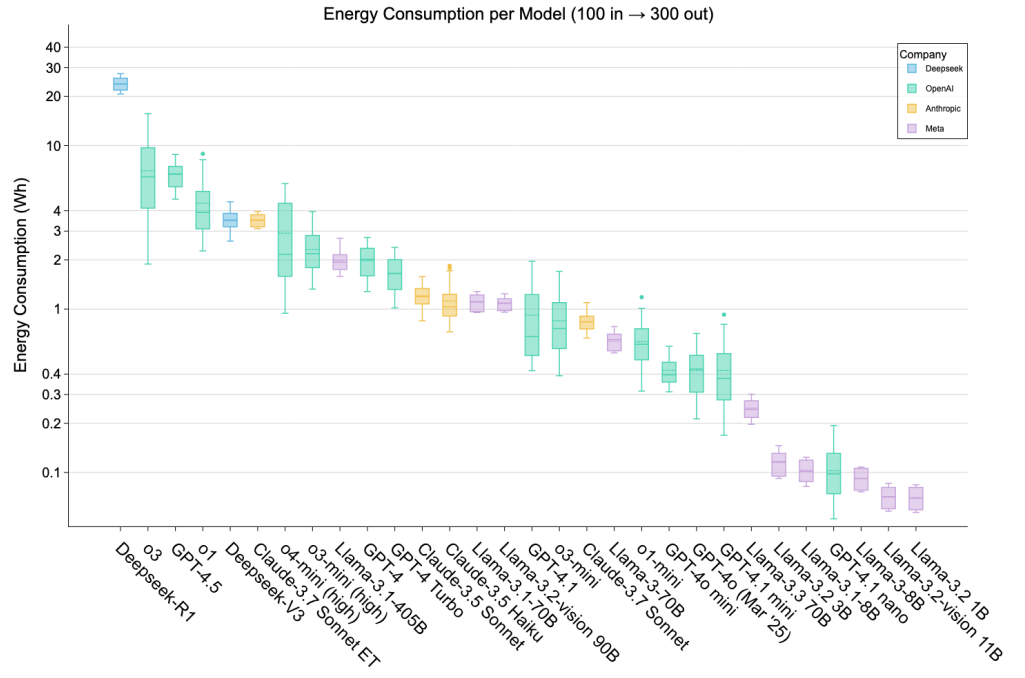
\includegraphics[width=\textwidth]{medium-size-consumption.png}
        \caption{Energy consumption for a small query (100 input tokens, 300 output tokens).}
        \label{fig:energy_consumption_small}
    \end{subfigure}
    \vskip 1em
    \begin{subfigure}[b]{0.8\textwidth}
        \centering
        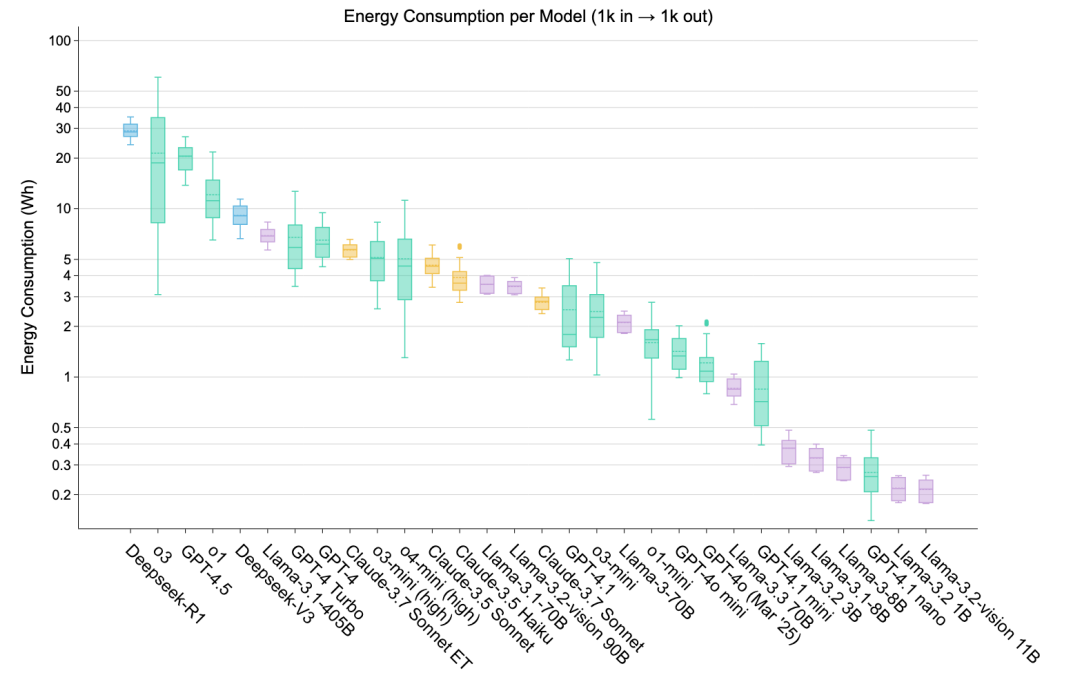
\includegraphics[width=\textwidth]{high-size-cosuption.png}
        \caption{Energy consumption for a large query (1000 input tokens, 1000 output tokens).}
        \label{fig:energy_consumption_large}
    \end{subfigure}
    \caption{Comparison of the energy consumption of different LLMs for small and large queries. The data highlights the significant increase in energy requirements as query size grows. These graphs have been sourced from \cite{hungry_ai}.}
    \label{fig:energy_consumption}
\end{figure}

\section{Scope}
While we've examined several critical challenges facing LLMs, it's worth emphasizing that these models hold significant potential for positive impact. As such, what was outlined in the previous sections points instead toward an urgent need for alternatives to the current paradigm of massive, centralized LLMs. A promising solution lies in compression techniques that can dramatically reduce model size while preserving core functionality. Through compression, billion-parameter server-sized models can be scaled down to more manageable ones that run much more efficiently.

\subsection{The main objective}
Given the context, the objective of this project is to push the boundaries of memory efficiency for small-scale LLMs by applying a targeted suite of compression techniques. We begin with a distilled model, a 1B parameter variant of LLaMA 3 \cite{llama3_1b}, which already represents a significantly reduced footprint compared to full-scale LLMs. From there, we explore and implement further optimizations, including depth and width pruning, \textit{Low-Rank Adaptation} (LoRA), and quantization.

Pruning allows us to remove redundant layers or neurons from the network architecture, trimming excess capacity without substantial loss of capability. Quantization reduces the bit-width of model weights and activations, decreasing both memory usage and compute requirements. LoRA, meanwhile, introduces a lightweight, parameter-efficient training mechanism that reduces the cost of fine-tuning and adaptation without (necessarily) modifying the base model weights. In this way, the model can be adapted to new tasks or domains with minimal overhead.

The reason behind the focus on maximizing memory efficiency is related to the fact that memory represents the most expensive constraint in our target deployment scenario, where the intended hardware platform consists of a low-power RISC-V SoC with severely constrained memory resources (further details on the target hardware can be found in Section \ref{target_hardware}). Crucially, optimizations that reduce memory footprint also translate directly into computational complexity improvements, creating a dual benefit for resource-constrained environments.

\subsection{How can optimization techniques help?}
Optimization techniques tackle the environmental, social, and infrastructure problems that come with large-scale LLMs. When models run more efficiently, they need far less power for each query. Smaller models can actually run on edge devices and other energy-efficient hardware, cutting down on electricity usage substantially. This efficiency boost also extends the useful life of older devices: hardware that might otherwise be considered obsolete can suddenly run modern LLMs, which helps reduce electronic waste and makes better use of existing resources.

There's also the autonomy angle. Compact models that run locally allows users to be independent from centralized servers when using AI. People can run LLMs right on their own devices without any internet connection, which means no data gets sent to third parties and there's no risk of surveillance. This approach supports decentralization and opens up AI access to areas with poor connectivity or limited economic resources.

In other words, optimization is a pathway toward environmentally sustainable, privacy-respecting, and widely accessible AI.


\section{Document structure}
Will write this when the document is finished.

\chapter{Linee guida architetturali}
\lhead[\fancyplain{}{\bfseries\thepage}]{\fancyplain{}{\bfseries\rightmark}}
% Chapter 2: Background and Related Work
Before explaining the details and implementation of the methodology used in the context of this thesis, it is essential to provide an overview of the evolution of the inner workings of the Transformer architecture as well as Language Models in general. In addition, in this chapter covers relevant optimization techniques and how they influenced the final result.
Finally, we will also shed some light on the target hardware, whose limitations have been a driving force behind the design choices made in this project.

\section{Early Language Models}
Before the emergence of the Transformer architecture, language models predominantly relied on \textit{Recurrent Neural Networks} (RNNs) . These networks represent an evolution of the \textit{Multi-Layer Perceptron} (MLP), incorporating cyclic connections within their architecture to create recurrent circuits. This design enables the network to maintain a form of memory, allowing it to consider previous inputs when generating predictions and thereby capturing long-range dependencies inherent in sequential data such as text.

Despite their theoretical advantages, RNNs suffer from a critical limitation known as the vanishing gradient problem \cite{rnn}. During backpropagation, throughout time, gradients from earlier steps diminish exponentially as they propagate backward through the network layers. This degradation severely hampers the network's ability to be trained effectively, as the influence of distant past information becomes negligible in the parameter updates.

To address these limitations, Hochreiter and Schmidhuber introduced \textit{Long Short-Term Memory} (LSTM) networks \cite{lstm}, which revolutionized sequence modeling through their sophisticated gating mechanisms. LSTMs employ specialized memory cells designed to selectively retain, update, and output information across extended sequences. The architecture incorporates three fundamental gate types that regulate information flow:
\begin{itemize}
    \item The \textit{input gate} determines the extent to which new information from the current input should be incorporated into the cell state. It evaluates the relevance of incoming data and controls its integration with existing memory.
    \item The \textit{forget gate} governs the retention of information from previous time steps, deciding which aspects of the historical cell state remain relevant and should be preserved.
    \item Finally, the \textit{output gate} regulates how much of the current cell state should be exposed to subsequent layers, effectively controlling what information propagates forward in the network.
\end{itemize}

This gating mechanism allows LSTMs to maintain gradient flow over much longer sequences compared to vanilla RNNs. Thus, they can capture dependencies spanning hundreds of time steps, making them particularly effective for tasks requiring long-term context understanding such as language modeling, machine translation, and text summarization. A visual representation of an LSTM cell is shown in Figure \ref{fig:lstm-architecture}.
\begin{figure}[!htbp]
\centering
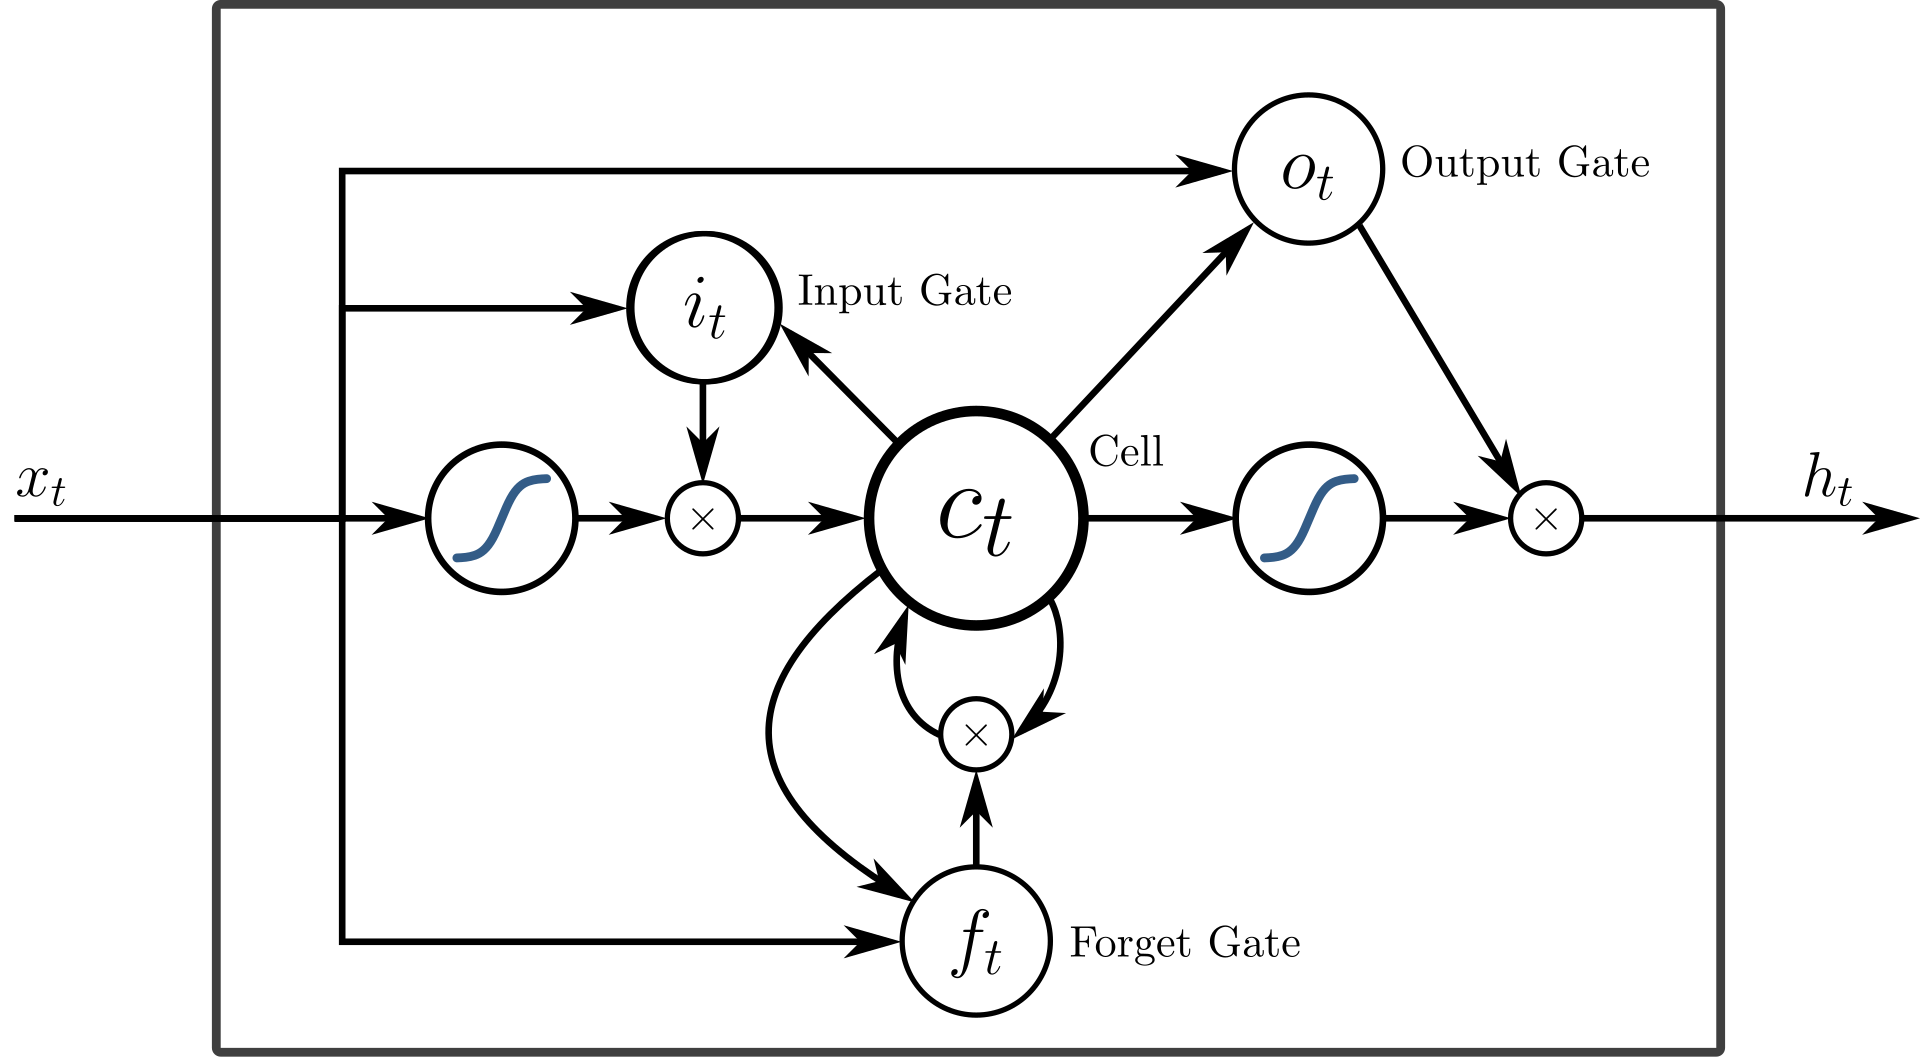
\includegraphics[width=0.7\textwidth]{image.png}
\caption{Architecture of an LSTM cell showing the three gating mechanisms. The input gate (left) controls information incorporation, the forget gate (center) manages memory retention, and the output gate (right) regulates information flow to subsequent layers. The cell state (horizontal line) maintains long-term memory throughout the sequence.}
\label{fig:lstm-architecture}
\end{figure}

While LSTMs significantly improved the ability to model sequential data, they still faced challenges in terms of parallelization and context understanding, especially when compared to Transformers.  Nevertheless, LSTMs are still widely used for various \textit{natural language processing} (NLP) tasks, including text generation \cite{lstm_textgeneration}.

\section{The Transformer Architecture}  \label{transformer_architecture}

The Transformer architecture, introduced by Vaswani et al. \cite{attention_is_all_you_need}, fundamentally changed how we approach sequence modeling by abandoning recurrent connections entirely in favor of attention mechanisms. Unlike LSTMs that process sequences step-by-step, the Transformer can examine all positions simultaneously, allowing for efficient parallelization during training. Moreover, it can capture long-range dependencies thanks to the attention mechanism.

\subsection{The Attention Mechanisms}

At the core of the Transformer lies the attention mechanism, which fundamentally changed how neural networks process sequential information. The attention mechanism addresses the information bottleneck created when sequence models compress an entire input sequence into a single fixed-size vector. This bottleneck becomes particularly problematic for long sequences, where important information can be lost or diluted.

Attention allows a model to dynamically focus on different parts of the input sequence when generating each output token, similar to how humans selectively concentrate on relevant information when reading or translating text. This is done, essentially, by directly comparing and relating any two positions in a sequence, regardless of their distance (i.e. self-attention). This selective focus mechanism enables the model to capture long-range dependencies more effectively and provides interpretable insights into which input elements influenced specific predictions.

\subsection{Scaled Dot-Product Attention Mechanics}

The Transformer's scaled dot-product attention operates on three matrices derived from the input:

\begin{equation}
\text{Attention}(Q, K, V) = \text{softmax}\left(\frac{QK^T}{\sqrt{d_k}}\right)V
\end{equation}

Each component serves a specific purpose:

\begin{itemize}
   \item \textbf{Queries (Q)}: Generated by $Q = XW_Q$ where $X$ is the input and $W_Q \in \mathbb{R}^{d_{\text{model}} \times d_k}$. Each query vector represents ``what information am I looking for?''
   \item \textbf{Keys (K)}: Generated by $K = XW_K$ where $W_K \in \mathbb{R}^{d_{\text{model}} \times d_k}$. Keys act as indexed labels for each position's content.
   \item \textbf{Values (V)}: Generated by $V = XW_V$ where $W_V \in \mathbb{R}^{d_{\text{model}} \times d_v}$. Values contain the actual information to be retrieved.
\end{itemize}

The attention computation proceeds in four steps:

\begin{enumerate}
   \item \textbf{Similarity Computation}: $QK^T$ produces a $n \times n$ matrix where entry $(i,j)$ represents how much position $i$ should attend to position $j$. The dot product naturally measures similarity between query and key vectors.

   \item \textbf{Scaling}: Division by $\sqrt{d_k}$ (where $d_k$ is the dimensionality of the keys) prevents the dot products from becoming too large. Without scaling, large dot products push the softmax function into regions with extremely small gradients. For example, if $d_k = 512$, dot products could reach magnitudes of $\pm 20$ or more, causing softmax to output distributions close to one-hot vectors.

   \item \textbf{Normalization}: The softmax function converts similarity scores into a probability distribution: $\text{softmax}(x_i) = \frac{e^{x_i}}{\sum_{j=1}^n e^{x_j}}$. This ensures attention weights sum to 1 and creates a differentiable selection mechanism.

   \item \textbf{Weighted Aggregation}: The attention weights are applied to the value vectors, producing a weighted sum that represents the attended information for each position.
\end{enumerate}

\subsection{Multi-Head Attention Architecture}

The Transformer employs multi-head attention so that each head can focus on different parts of the input. Some heads might track syntax, others semantics, positions, etc. This is done by projecting the input matrices $Q, K, V$ by $h$ times using different learned linear projections:
\begin{equation}
(QW_i^Q, KW_i^K, VW_i^V)
\end{equation}
Given this, each head is computed as:
\begin{equation}
\text{head}_i = \text{Attention}(QW_i^Q, KW_i^K, VW_i^V)
\end{equation}
As such, the final equation for multi-head attention is:
\begin{equation}
\text{MultiHead}(Q, K, V) = \text{Concat}(\text{head}_1, \ldots, \text{head}_h)W^O
\end{equation}

Each head uses different projection matrices $W_i^Q \in \mathbb{R}^{d_{\text{model}} \times d_k}$, $W_i^K \in \mathbb{R}^{d_{\text{model}} \times d_k}$, and $W_i^V \in \mathbb{R}^{d_{\text{model}} \times d_v}$, where typically $d_k = d_v = d_{\text{model}}/h$ for $h$ heads. 

Multi-head attention essentially gives the model multiple different perspective of the same input, and it is a vital system that contributes to make this architecture so powerful.

\subsection{Positional Information Integration}

Since attention is permutation-invariant, the Transformer requires explicit positional information. The original work uses sinusoidal positional encodings:

\begin{align}
PE_{(\text{pos}, 2i)} &= \sin(\text{pos}/10000^{2i/d_{\text{model}}}) \\
PE_{(\text{pos}, 2i+1)} &= \cos(\text{pos}/10000^{2i/d_{\text{model}}})
\end{align}

These encodings have useful properties: they create unique representations for each position, allow the model to learn relative positions through linear combinations, and can theoretically handle sequences longer than those seen during training.

This architecture enables the Transformer to model dependencies between any pair of positions with constant path length, while maintaining full parallelizability during training.

\subsection{Encoder-Decoder Transformers}

Transformer-based models generate text by predicting the next token in a sequence, conditioned either on an external input (encoder-decoder models) or on the sequence generated so far (decoder-only models). The former is what the original Transformer architecture~\cite{attention_is_all_you_need} follows.

\begin{itemize}
  \item The \textbf{encoder} processes the full input sequence in parallel, producing a series of contextual embeddings that capture the meaning and structure of the input tokens.
  \item The \textbf{decoder} generates the output sequence token by token, using the embeddings from the encoder.
\end{itemize}

This design enables the model to generate outputs that are grounded in the input sequence, rather than generating new text from scratch. As such, it is well-suited for sequence-to-sequence tasks such as machine translation.

\subsection{Decoder-Only Transformers}

In decoder-only Transformers, there is no separate encoder module. The model predicts each token based only on the previously generated tokens, modeling the joint distribution \( p(x_1, x_2, \ldots, x_n) \) autoregressively. This means that the model outputs one token at a time, appends it to the input, and repeats until a stopping condition is met.

These models are simpler and more scalable, and they are the ones employed in large language models such as GPT \cite{gpt}, and of course LLaMA \cite{llama}.

Decoder-only architectures are ideal for open-ended text generation and other tasks where the output is not conditioned on a separate input sequence.
Figure \ref{fig:sidebyside} shows a comparison of encoder-decoder and decoder-only transformer architectures.

\section{The LLaMA family of models}

The \textit{Large Language Model Meta AI} (LLaMA) family~\cite{llama3}, developed by Meta AI, comprises a series of transformer-based autoregressive language models designed as competitors to OpenAI's GPT model family. The original LLaMA models were introduced in early 2023, followed by LLaMA 2 \cite{llama2} later that year and LLaMA 3 in 2024.

The models vary in the number of parameters and capabilities, with the newer versions offering improved performance over the older ones. In particular, with LLaMA 3, Meta introduced models at 8B and 70B parameters with major upgrades in both training scale and performance over LLaMA 2, while approaching results to OpenAI's GPT-4 \cite{gpt4} \cite{llama3}.

The main feature of LLaMA, however, is its open-weight release strategy. Unlike most proprietary models, Meta provides access to the model weights under a research-friendly license, enabling the broader research community and industry practitioners to experiment with, fine-tune, and deploy large-scale language models without relying on closed systems. This openness has led to a proliferation of derivative models, and of course the making of the project described in this document.


\begin{figure}[htbp]
    \centering
    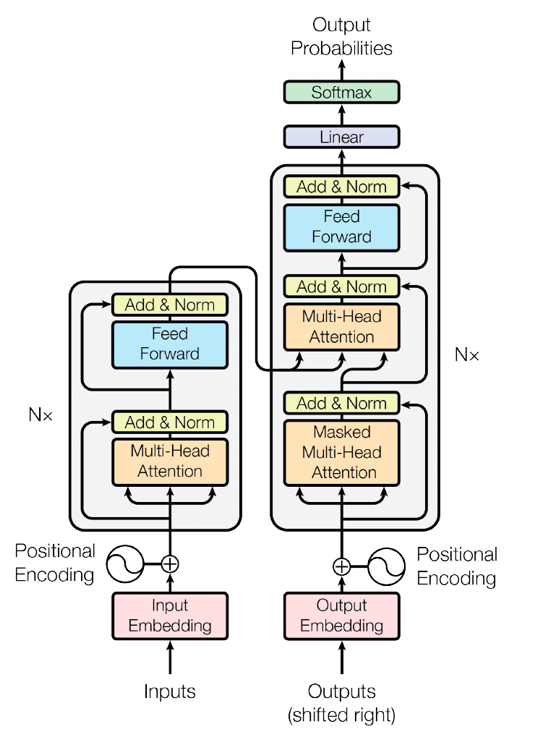
\includegraphics[width=0.45\textwidth]{transformer.png}
    \hfill
    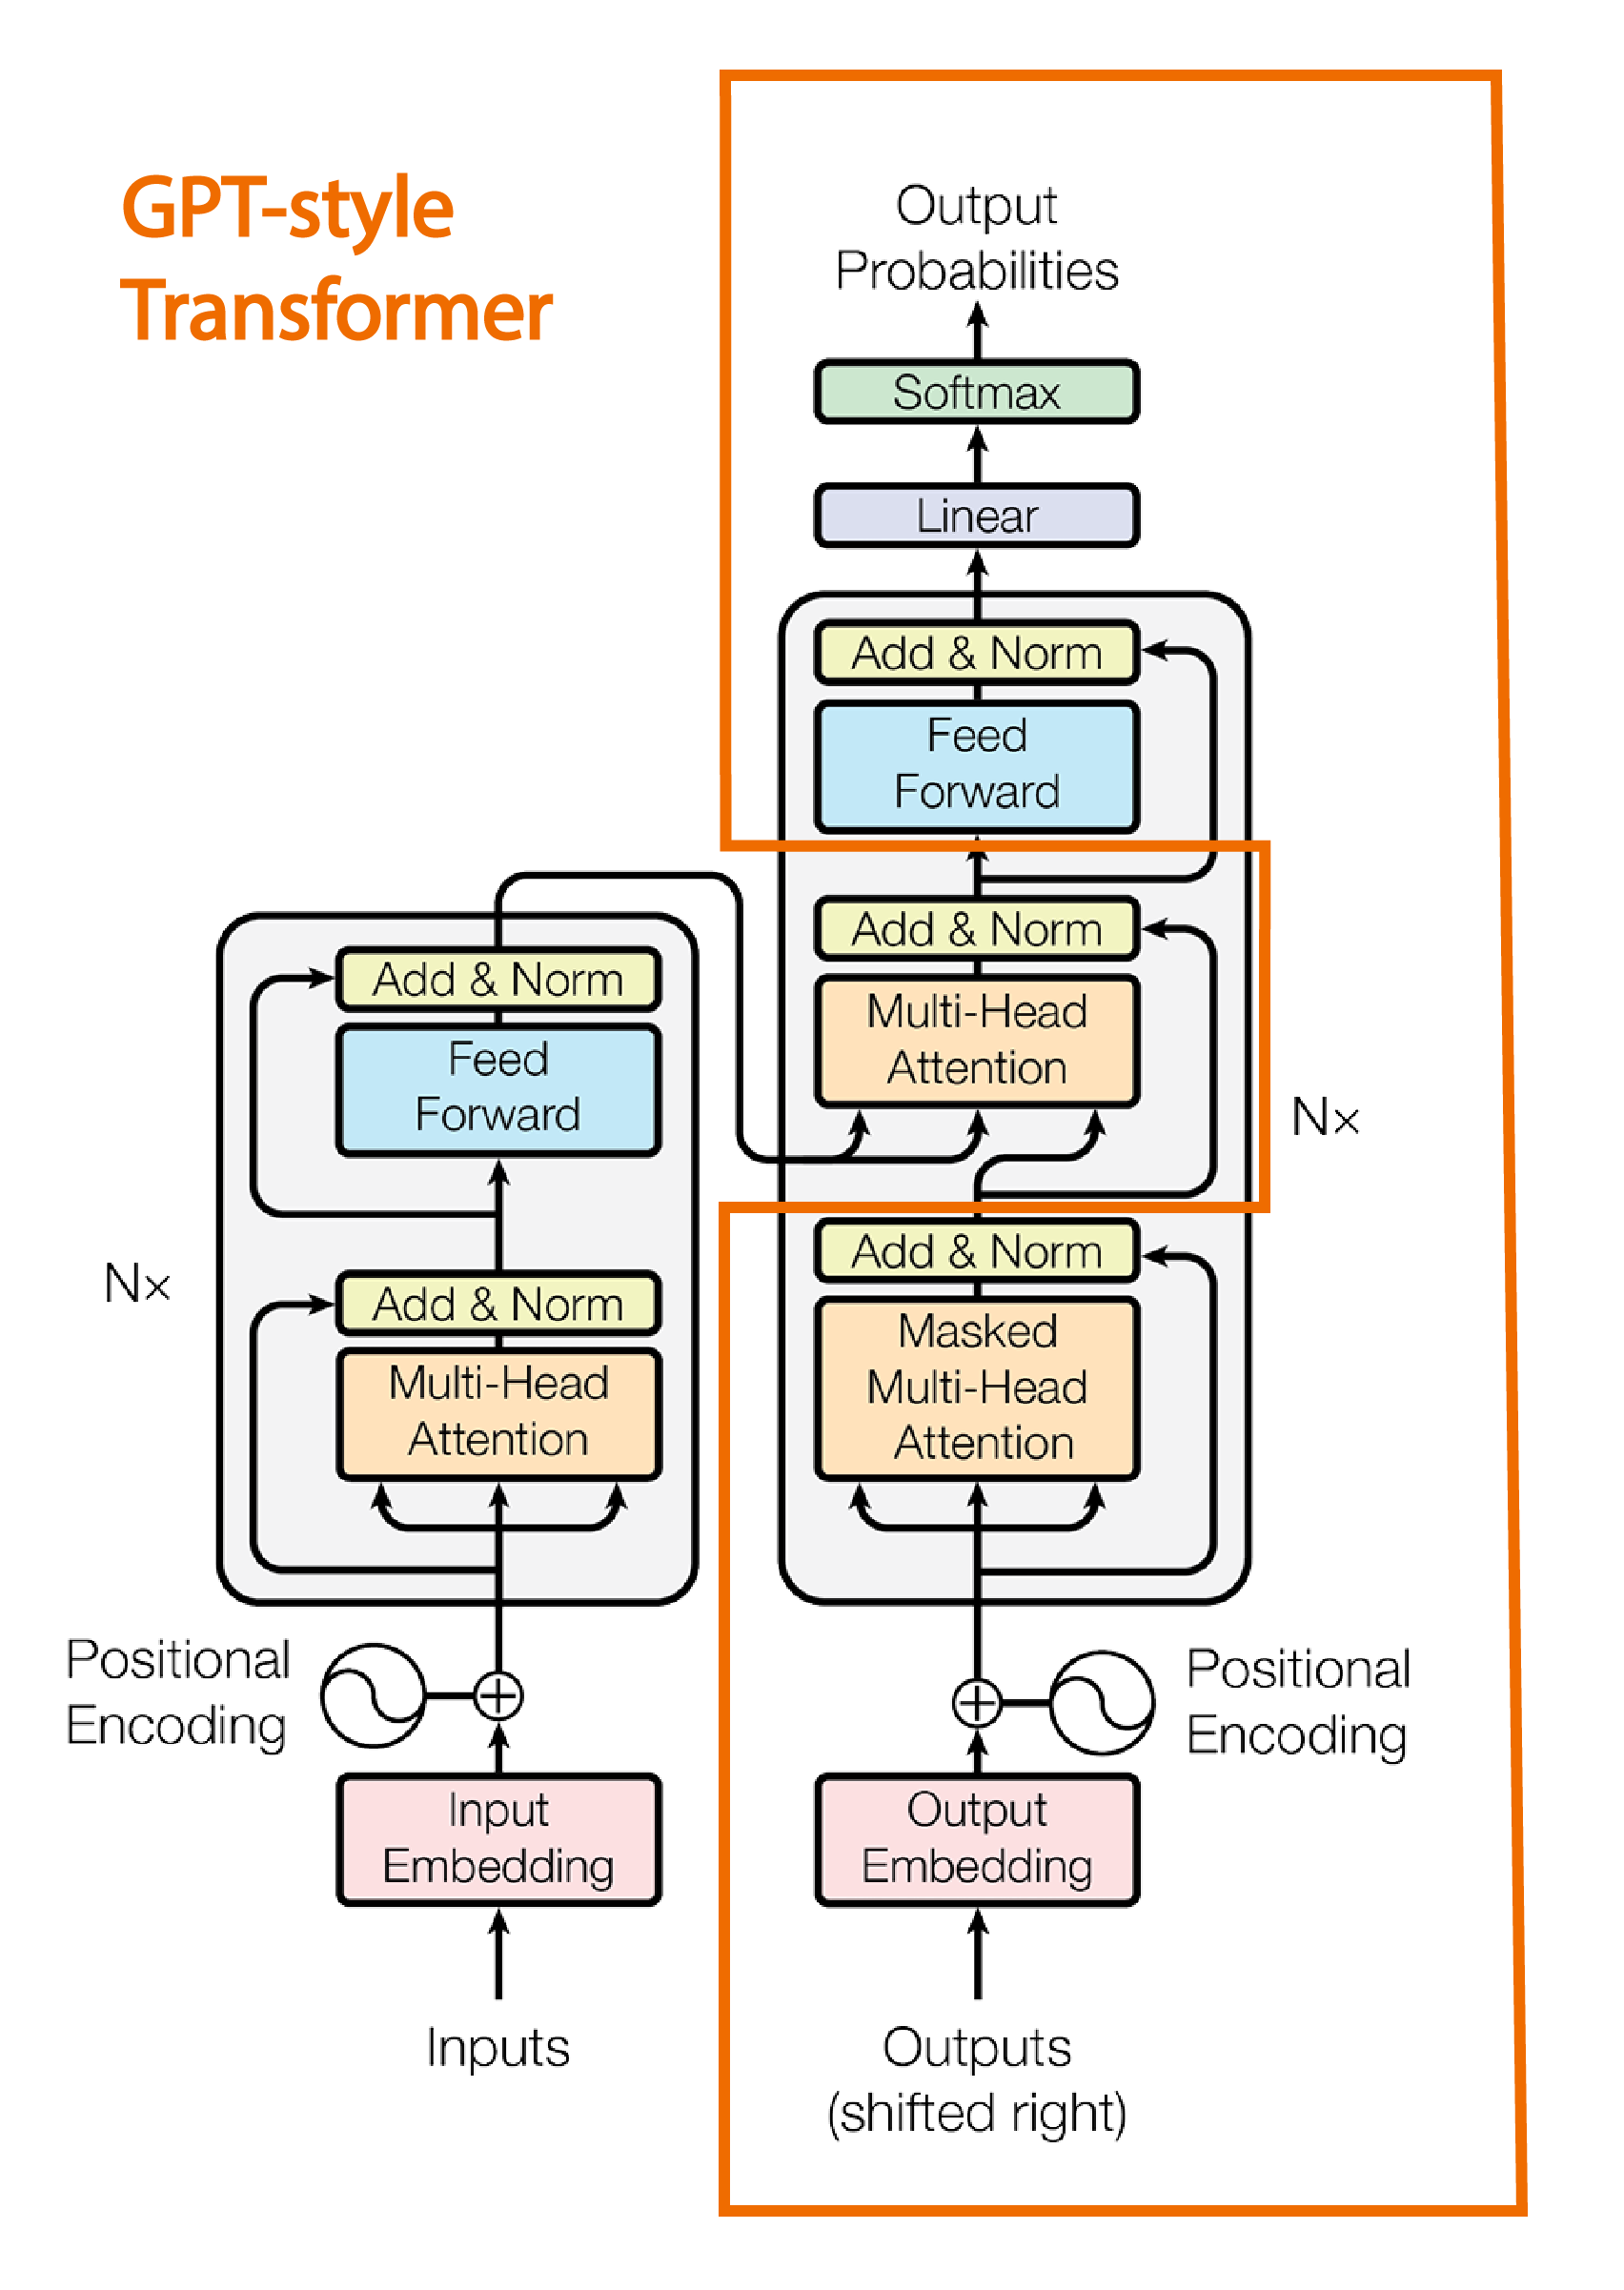
\includegraphics[width=0.45\textwidth]{transformer-gpt.png}
    \caption{On the left, a standard Transformer architecture, which consists of an encoder and a decoder. On the right, we can observe the same architecture, while highlighting the only the layers used by a GPT-style model, which is a decoder-only transformer. The main difference is that the decoder does not attend to the encoder's output, allowing for auto-regressive generation.}
    \label{fig:sidebyside}
\end{figure}

\section{A look at the target hardware} \label{target_hardware}

\section{Relevant compression and optimization techniques}
speak about distillation, paper about width+depth pruning.




\chapter{Implementazione}
\lhead[\fancyplain{}{\bfseries\thepage}]{\fancyplain{}{\bfseries\rightmark}}
Having covered the importance of LLM optimization and the technical architecture of transformers in previous chapters, we now turn to the practical challenge of model compression.

This chapter begins with preliminary experiments on layer manipulation that revealed crucial insights about architectural redundancy in transformer models and shaped the main compression strategy. The chapter then presents what is possibly the heart of this research: a multi-stage pipeline that combines several optimization techniques in a structured sequence. Each stage is examined with both theoretical foundations and practical implementation details. Finally, the evaluation methods and their underlying motivation are detailed.

\section{Preliminary Research: Franken-LLaMA} \label{frankenllama}

Before embarking on systematic compression techniques for our target 1B parameter LLaMA model, we conducted preliminary research to understand the behavior of transformer architectures under structural modifications. This exploratory consisted on the ``Franken-LLaMA'' project \cite{franken-llama}, which involved experimenting with selective layer skipping and repetition in the larger LLaMA2-7B-Chat \cite{llama2} model to gain a first insight into which components of the transformer architecture are most critical for maintaining model performance.

The approach centered on modifying the standard transformer execution flow by selectively including, excluding, or repeating attention blocks within the 32-layer architecture. The repetition strategy was particularly attractive as it could theoretically reduce memory footprint by reusing the same layer weights multiple times rather than storing distinct parameters for each position. This weight sharing approach aligned directly with the target hardware constraints outlined in Section \ref{target_hardware}, where the memory limitation makes parameter reduction a critical optimization target.

25 different layer configurations were tested, each of which was evaluated through qualitative text generation tasks and quantitative assessment on the HellaSwag dataset \cite{hellaswag}.
The results revealed several that conservative modification, often maintained reasonable performance while reducing computational overhead. In particular, skipping the layers more towards the middle of the model rather than its ends resulted in low performance degradation. For instance, the configuration that skipped layers 23-27 achieved a HellaSwag score of 0.38 compared to the baseline's 0.34, suggesting that certain middle layers may contribute less to final performance than expected.

However, more aggressive modifications typically led to severe degradation in output quality. Configurations involving extensive layer repetition or using only sparse layer selections often produced incoherent text with non-ASCII characters and semantic breakdown. This behavior indicated that while some redundancy exists in the transformer architecture, maintaining a balanced representation across different depths remains crucial for coherent language generation.

These preliminary findings informed the subsequent approach to systematic compression: it revealed that strategic layer removal could sometimes improve performance metrics, suggesting that pruning techniques might offer promising avenues for optimization; at the same time, it showed how layer repetition was not a viable strategy and caused heavy performance degradation.

\section{An Overview of the Pipeline}

The core result of this research is the compression pipeline, which implements a sequential approach that combines multiple optimization techniques in a carefully orchestrated manner. As previously mentioned, the target model for these optimizations is LLaMA 3.2 1B, a distilled version of the larger LLaMA 3.2 model that has already undergone some level of pruning during its creation, according to the Hugging Face model documentation \cite{llama3_1b}.

The choice of this particular model as the starting point is both strategic and practical. While incorporating distillation directly into the pipeline would have been ideal given its effectiveness as a compression technique, the computational requirements make it rather prohibitive. Distillation essentially requires training a model from scratch, demanding extensive GPU resources that far exceed the computational budget available for the project. Thus, an existing pre-distilled model was utilized instead which already provides a compact yet capable foundation.

The pipeline follows a five-stage progression, with each stage building upon the previous one. The particular ordering was chosen based on the complementary nature of these techniques and their relative impact on model structure.

\begin{enumerate}
    \item The first stage implements depth-wise pruning (Section \ref{depth_pruning}), where entire transformer layers are removed based on importance metrics computed during a calibration phase. This coarse-grained approach eliminates redundant blocks, and ultimately redefines the skeleton of the architecture.

    \item Width-wise pruning follows as the second stage (Section \ref{wanda}), applying the WANDA algorithm to remove less critical weights within the remaining layers. This is a finer-grained approach compared to the depth-pruning, as it operates at the parameter level.

    \item The third stage introduces \textit{Low-Rank Adaptation} (LoRA) (Section \ref{lora}) to recover performance lost during the pruning phases, while also allowing for fine-tuning on specific downstream tasks.

    \item The fourth stage applies 4-bit quantization using GPTQ, reducing the memory footprint of individual parameters.

    \item The final stage includes an optional \textit{Eigenspace Low-Rank Approximation} (EoRA) step to improve the performance of the quantized model.
\end{enumerate}

Detailed descriptions of each stage are provided in the following sections. Each step yields an intermediate model suitable for independent evaluation, except when explicitly stated otherwise. The modular design supports selective execution through comprehensive tuning options, such as the ability to skip specific stages or experiment with different parameter configurations without modifying the core implementation. Having intermediate models allows to conduct ablation studies more easily and adapt the pipeline to specific hardware constraints.

\section{Depth-wise Pruning} \label{depth_pruning}

Depth pruning represents a structured approach to neural network compression that targets the architectural dimension of model depth rather than individual parameter elimination. Unlike width pruning, which reduces the size of weight matrices by removing neurons or attention heads while preserving the total number of layers, depth pruning removes entire layers or blocks from the network architecture. In the context of transformer-based language models, this typically involves eliminating complete attention blocks, each containing both a multi-head attention module and feed-forward network components. Figure \ref{fig:pruning_comparison} shows a visual comparison between the two pruning techniques.

\begin{figure}[htbp]
    \centering
    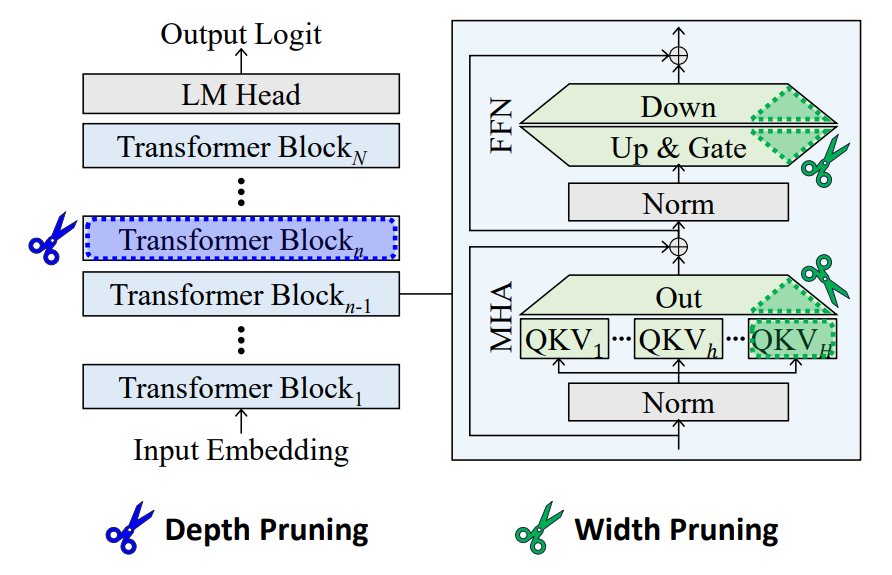
\includegraphics[width=0.7\textwidth]{pruning.png}
    \caption[Comparison of Depth and Width Pruning]{In depth pruning, we remove the single transformer layers (left). On the other hand, in width pruning we remove single neurons from the weight matrices (right). The image was sourced from \cite{shortened_llama}.}
    \label{fig:pruning_comparison}
\end{figure}

The depth pruning approach follows the methodology established by Kim et al. in their Shortened LLaMA work \cite{shortened_llama}, which demonstrated that removing entire transformer blocks can achieve competitive performance while delivering significant inference speedups, particularly under memory-constrained conditions. Rather than reducing individual weight dimensions as in width pruning, depth pruning eliminates entire layers from the model architecture, creating a more direct path to computational savings.

The depth pruning process begins with calculating layer importance scores using one of several metrics implemented in the pipeline. Three primary importance calculation methods are supported: magnitude-based scoring, Taylor expansion-based gradient analysis, and perplexity-based evaluation. The magnitude approach computes the L1 norm of weights within each transformer block, providing a simple baseline for layer significance. The Taylor method leverages first-order gradient information to estimate the impact of layer removal on model performance, following the approximation $L(W = 0) \approx L(W) + \nabla L \cdot (-W)$ where the gradient-weight product indicates layer importance. The perplexity method evaluates each layer by temporarily removing it and measuring the resulting degradation in language modeling performance on a calibration dataset.

Following the insights from Shortened LLaMA, the implementation protects the first four and last two layers from pruning, as these positions have been shown to be critical for maintaining performance (which is in line with what was discovered in Section \ref{frankenllama}). The remaining layers are ranked according to their importance scores, with the least significant layers selected for removal.

The removal process involves creating a new model architecture with the selected layers entirely eliminated, maintaining the original transformer structure for the remaining blocks. This approach contrasts sharply with width pruning techniques that create sparse weight matrices, as depth pruning produces models with clean, dense architectures that map naturally onto hardware accelerators without requiring specialized sparse computation support.

The implementation extends the Shortened LLaMA approach by integrating it into a comprehensive compression pipeline, where depth pruning serves as the foundation for subsequent optimization techniques. The layer importance calculations are performed efficiently using calibration datasets, typically requiring only 10 samples from standard corpora to produce reliable importance rankings. This efficiency makes depth pruning particularly attractive for resource-constrained scenarios where extensive calibration is impractical.

\section{Width-wise Pruning} \label{wanda}

Following depth-wise pruning, the second stage of the compression pipeline applies width-wise pruning. As mentioned in Section \ref{depth_pruning}, it operates at the parameter level, eliminating individual weights within the remaining layers to achieve fine-grained compression. Width pruning can be either:
\begin{itemize}
    \item \textbf{Unstructured}:
    \item \textbf{Structured}:
\end{itemize}

\subsection{WANDA Algorithm Overview}

WANDA introduces a novel pruning metric that combines weight magnitudes with input activation statistics to determine parameter importance. The core insight behind this approach stems from the observation that large language models exhibit emergent large magnitude features in their hidden states—outlier activations that are significantly larger than typical values and are crucial for model performance.

The WANDA importance metric for each weight $W_{ij}$ is defined as:

\begin{equation}
S_{ij} = |W_{ij}| \cdot \|X_j\|_2
\end{equation}

where $|W_{ij}|$ represents the absolute value of the weight and $\|X_j\|_2$ evaluates the L2 norm of the $j$-th input feature across all calibration samples. This formulation addresses a key limitation of traditional magnitude-based pruning: it fails to account for input activations, which play an equally important role in determining neuron outputs, especially in the presence of large magnitude features.

\subsection{Structured N:M Sparsity Implementation}

While WANDA was originally designed for unstructured sparsity, the compression pipeline implements its structured variant to leverage hardware acceleration capabilities. Specifically, the implementation focuses on structured N:M sparsity patterns, where at most N out of every M consecutive weights are non-zero.

The structured pruning process operates as follows:

\begin{enumerate}
   \item \textbf{Importance Calculation}: For each linear layer, compute the WANDA metric for all weights using calibration data
   \item \textbf{Grouping}: Organize weights into groups of M consecutive elements within each output channel
   \item \textbf{Selection}: Within each group, identify the N weights with the highest importance scores
   \item \textbf{Pruning}: Set the remaining (M-N) weights to zero
\end{enumerate}

This structured approach enables the use of specialized hardware accelerators, such as NVIDIA's sparse tensor cores, which can efficiently handle N:M sparsity patterns during inference.

\subsection{Implementation Details}

The WANDA implementation integrates seamlessly into the compression pipeline through the \texttt{prune\_wanda} function. Key implementation aspects include:

\textbf{Calibration Setup}: The algorithm uses the same calibration dataset as the depth pruning stage, typically consisting of 10 samples from the C4 corpus, ensuring consistency across optimization stages.

\textbf{Layer-wise Processing}: WANDA processes each transformer layer sequentially, updating activations after each layer is pruned to ensure that subsequent layers receive realistic input distributions.

\textbf{Per-output Comparison}: Following the original WANDA methodology, weights are compared and pruned on a per-output basis rather than globally across the layer. This approach maintains balanced pruning ratios across different output features, which proves crucial for preserving model performance.

\textbf{Binary Search for Sparsity}: For the variant implementation, a binary search algorithm finds the optimal threshold parameter $\alpha$ that achieves the target sparsity ratio while maximizing the cumulative importance of retained weights.

\subsection{Advantages and Computational Efficiency}

WANDA offers several advantages over more complex pruning methods:

\begin{itemize}
   \item \textbf{Single Forward Pass}: Unlike methods requiring iterative weight updates, WANDA completes pruning in a single forward pass through the model
   \item \textbf{No Weight Updates}: The algorithm requires no modifications to the remaining weights, suggesting that effective sparse subnetworks exist within the original model
   \item \textbf{Low Computational Overhead}: With $O(d^2)$ complexity compared to $O(d^3)$ for second-order methods, WANDA provides significant computational savings
   \item \textbf{Hardware Compatibility}: The structured N:M variant directly maps to accelerator capabilities without requiring specialized sparse computation libraries
\end{itemize}

The integration of WANDA as the width pruning stage creates a foundation for subsequent optimization techniques while maintaining the model's core functionality. The structured sparsity patterns ensure that the compressed model can benefit from hardware acceleration during inference, making this approach particularly suitable for deployment scenarios with strict performance requirements.
\section{LoRA} \label{lora}
\section{Quantization and EoRA} \label{quantization}
\section{Evaluation}

\chapter{Gestione dell'autenticazione}
\lhead[\fancyplain{}{\bfseries\thepage}]{\fancyplain{}{\bfseries\rightmark}}

% Chapter 4: Results and Analysis

This chapter presents the empirical evaluation of the pipeline that was described in Chapter \ref{chap:methodology} when applied to the LLaMA 3.2 1B Instruct model. The experiments reveal systematic patterns in how different optimization techniques affect performance across multiple evaluation metrics.

Subsequent sections examine compression efficiency, quality degradation, and the interaction effects between sequential optimization stages. Results demonstrate that certain technique combinations achieve substantial parameter reduction while maintaining acceptable capability levels, whereas others exhibit rapid degradation beyond critical compression ratios.

The tables presented in this chapter display a representative subset of the experimental data to highlight key findings and trends. The complete results from all configurations that were tested are available in Appendix \ref{app:appendix1}, along with examples of text generated by selected models.

\section{Pruning Analysis}

The initial phase of experimentation examined the isolated effects of pruning techniques without quantization or recovery mechanisms. A total of 42 pruning-only configurations were evaluated, including 29 combined ones that applied both depth and width pruning simultaneously to assess the compounding effects of multi-dimensional compression.

The results shown in Table \ref{tab:depth_pruning_results} demonstrate a steep degradation curve where even modest layer removal causes substantial quality deterioration. The most striking observation is the precipitous decline beyond removing two layers. While Depth 2, the variant with 2 layers removed, maintains reasonable functionality with 53.0\% accuracy on TriviaQA's open-book benchmark (i.e. TriviaQA Open) compared to the baseline's 81.8\%, removing four layers causes performance to collapse to just 14.2\%. This suggests that architectural depth in transformer models exhibits critical thresholds beyond which fundamental language capabilities deteriorate rapidly.

{\begin{table}[htbp]
\centering
\footnotesize
\caption[Results for Pruning-Only Configurations (Subset)]{Results for models which have undergone pruning without quantization or performance recovery. This table presents a subset of results from the complete dataset available in Appendix \ref{app:appendix1}.} \label{tab:pruning_only_results}
\label{tab:depth_pruning_results}
\begin{tabular}{lcccccc}
\hline
\textbf{Config} & \multicolumn{2}{c}{\textbf{TriviaQA (\%) $\uparrow$}} & & \textbf{WikiText $\downarrow$} & \textbf{\#Params} & \textbf{Size} \\
\cline{2-3}
& \textbf{Closed} & \textbf{Open} & & \textbf{PPL} & & \textbf{(GB)} \\
\hline
Baseline Instruct & 50.6 & 81.8 & & 26.61 & 1235.8M & 2.30 \\
Depth 2 & 20.0 & 53.0 & & 55.24 & 1114.2M & 2.08 \\
Depth 4 & 5.6 & 14.2 & & 230.77 & 992.5M & 1.85 \\
Depth 6 & 2.0 & 2.4 & & 2081.04 & 870.9M & 1.62 \\
Depth 8 & 1.2 & 1.4 & & 227734.90 & 749.2M & 1.40 \\
Width 1:2 & 1.8 & 2.2 & & 471.66 & 749.3M & 2.30 \\
Width 2:4 & 7.0 & 17.2 & & 161.10 & 749.3M & 2.30 \\
Width 1:8 & 47.8 & 80.8 & & 27.19 & 1114.2M & 2.30 \\
Width 4:8 & 12.6 & 42.4 & & 81.32 & 749.3M & 2.30 \\
Width 1:16 & 49.2 & 81.8 & & 26.77 & 1175.0M & 2.30 \\
Width 8:16 & 16.2 & 52.8 & & 64.08 & 749.3M & 2.30 \\
Width 12:16 & 0.2 & 0.2 & & 1793.97 & 506.0M & 2.30 \\
Depth 2 + Width 1:2 & 0.4 & 0.4 & & 694.34 & 688.4M & 2.08 \\
Depth 2 + Width 2:4 & 3.8 & 5.0 & & 309.32 & 688.4M & 2.08 \\
Depth 2 + Width 1:8 & 20.2 & 53.6 & & 57.22 & 1007.7M & 2.08 \\
Depth 2 + Width 4:8 & 6.4 & 15.2 & & 185.43 & 688.4M & 2.08 \\
Depth 2 + Width 1:16 & 19.6 & 51.6 & & 55.68 & 1061.0M & 2.08 \\
Depth 2 + Width 8:16 & 7.6 & 23.4 & & 139.97 & 688.4M & 2.08 \\
Depth 4 + Width 1:8 & 5.2 & 14.8 & & 244.69 & 901.3M & 1.85 \\
Depth 4 + Width 4:8 & 3.0 & 2.6 & & 774.60 & 627.6M & 1.85 \\
Depth 4 + Width 1:16 & 4.6 & 14.6 & & 235.32 & 946.9M & 1.85 \\
Depth 4 + Width 8:16 & 2.6 & 6.2 & & 591.59 & 627.6M & 1.85 \\
Depth 6 + Width 1:8 & 2.0 & 1.6 & & 2376.63 & 794.9M & 1.62 \\
Depth 6 + Width 4:8 & 0.8 & 1.0 & & 77482.90 & 566.8M & 1.62 \\
Depth 6 + Width 1:16 & 1.8 & 1.6 & & 2032.84 & 832.9M & 1.62 \\
Depth 8 + Width 4:8 & 0.8 & 0.4 & & 554910.71 & 506.0M & 1.40 \\
Depth 8 + Width 3:4 & 0.4 & 0.4 & & 1044840.71 & 384.3M & 1.40 \\

\hline
\end{tabular}
\end{table}
}

The perplexity measurements on WikiText-2 reinforce this pattern, with Depth 2 showing a manageable increase to 55.24 compared to the baseline's 26.61, while deeper pruning leads to catastrophic degradation. Removing eight layers (Depth 8 configuration) causes perplexity to exceed beyond 200,000, indicating near-complete loss of coherent language modeling capability.

On the other hand, width pruning shows markedly different characteristics. The Width 1:8 variant emerges as particularly noteworthy, maintaining 80.8\% accuracy on TriviaQA Open while reducing parameters from 1235.8M to 1114.2M. This represents only a minimal performance drop of 1.0 percentage point while achieving a 10\% reduction in model size, with parameter count comparable to the Depth 2 configuration. The perplexity increase is equally modest, rising from 26.61 to 27.19. This finding suggests that transformer architectures contain significant redundancy in their width dimension when weights are removed judiciously, with the WANDA algorithm's ability to identify and remove less critical weights while preserving essential model capacity proving effective for moderate compression ratios.

However, more aggressive width pruning follows the same catastrophic degradation pattern observed when extensively removing entire layers. The Width 1:2 configuration reduces TriviaQA Open accuracy to just 2.2\%, thus proving that there are clear limits to how extensively models can be compressed through width reduction alone.
Moreover, the granularity of width pruning significantly influences these results, as evidenced by the progression from Width 1:2 (2.2\% TriviaQA Open) to Width 2:4 (17.2\%) to Width 4:8 (42.4\%), showing how different sparsity patterns at the same compression ratio yield vastly different outcomes.

ultimately, performance of models with combined configurations, without recovery mechanisms, proves unacceptable for practical deployment unless weight removal remains minimal. The only viable exception is Depth 2 + Width 1:8, which maintains 53.6\% accuracy on TriviaQA Open while achieving an 18\% parameter reduction, representing the practical threshold for structural compression without additional optimization techniques.

\section{Complete Pipeline Performance}

Of the 42 pruned-only configurations, 27 were selected to undergo LoRA fine-tuning and quantization. In particular, training was conducted separately on both WikiText and TriviaQA train datasets using 8192 samples divided into batches of 8. Additionally, 12 of these variants also underwent EoRA performance recovery to assess its effectiveness in mitigating quantization-induced degradation. Table \ref{tab:complete_pipeline_results} presents key configurations that showcase different aspects of the optimization process.

{\footnotesize
\begin{table}[htbp]
\centering
\footnotesize
\caption[Results for Complete Pipeline Configurations (Subset)]{Results for models which have undergone the complete optimization pipeline or selected steps in addition to pruning. This table presents a subset of results from the complete dataset available in Appendix \ref{app:appendix1}.} \label{tab:complete_pipeline_results}
\begin{tabular}{lcclcccc}
\hline
\textbf{Config} & \textbf{LoRA} & \textbf{Quant} & & \multicolumn{2}{c}{\textbf{TriviaQA (\%) $\uparrow$}} & \textbf{WikiText $\downarrow$} & \textbf{Size} \\
\cline{5-6}
& \textbf{Type} & & & \textbf{Closed} & \textbf{Open} & \textbf{PPL} & \textbf{(GB)} \\
\hline
Depth 2 & TriviaQA & No & & 27.8 & 60.2 & 51.09 & 2.08 \\
Depth 2 & TriviaQA & Yes & & 23.9 & 54.6 & 55.03 & 0.92 \\
Depth 2 & TriviaQA & EoRA & & 24.4 & 58.4 & 54.60 & 0.92 \\
Width 1:2 & WikiText & No & & 10.0 & 32.0 & 40.26 & 2.30 \\
Width 1:2 & WikiText & Yes & & 9.1 & 27.3 & 42.19 & 0.98 \\
Width 1:2 & WikiText & EoRA & & 8.8 & 28.3 & 41.78 & 0.98 \\
Width 1:2 & TriviaQA & No & & 12.4 & 29.3 & 145.54 & 2.30 \\
Width 1:2 & TriviaQA & Yes & & 11.3 & 26.5 & 154.33 & 0.98 \\
Width 1:2 & TriviaQA & EoRA & & 11.7 & 25.7 & 152.53 & 0.98 \\
Width 1:8 & WikiText & No & & 47.8 & 80.8 & 15.70 & 2.30 \\
Width 1:8 & WikiText & Yes & & 39.0 & 74.8 & 16.85 & 0.98 \\
Width 1:8 & TriviaQA & EoRA & & 42.0 & 77.2 & 32.86 & 0.98 \\
Width 4:8 & WikiText & No & & 17.0 & 51.1 & 26.04 & 2.30 \\
Width 4:8 & WikiText & Yes & & 15.7 & 45.3 & 27.40 & 0.98 \\
Width 8:16 & TriviaQA & Yes & & 20.8 & 55.7 & 60.67 & 0.98 \\
Width 8:16 & WikiText & Yes & & 17.5 & 52.1 & 25.39 & 0.98 \\
Width 8:16 & WikiText & EoRA & & 17.8 & 54.9 & 25.09 & 0.98 \\
Depth 2 + Width 1:8 & WikiText & EoRA & & 22.3 & 59.6 & 22.98 & 0.92 \\
Depth 2 + Width 1:8 & TriviaQA & No & & 27.4 & 60.4 & 51.89 & 2.08 \\
Depth 2 + Width 1:16 & TriviaQA & Yes & & 25.2 & 56.3 & 55.46 & 0.92 \\
Depth 2 + Width 2:4 & WikiText & Yes & & 10.6 & 30.8 & 41.54 & 0.92 \\
Depth 2 + Width 2:4 & WikiText & EoRA & & 10.4 & 29.8 & 40.73 & 0.92 \\
Depth 4 + Width 1:16 & WikiText & No & & 18.1 & 53.2 & 29.51 & 1.85 \\
Depth 4 + Width 1:16 & WikiText & Yes & & 15.2 & 48.6 & 31.66 & 0.86 \\
Depth 4 + Width 1:16 & TriviaQA & No & & 18.7 & 47.3 & 89.32 & 1.85 \\
Depth 4 + Width 2:4 & WikiText & Yes & & 7.2 & 25.8 & 52.20 & 0.86 \\
Depth 4 + Width 2:4 & WikiText & EoRA & & 7.6 & 26.3 & 51.19 & 0.86 \\
Depth 4 + Width 4:8 & WikiText & Yes & & 8.2 & 29.6 & 46.34 & 0.86 \\
Depth 4 + Width 4:8 & WikiText & EoRA & & 8.3 & 31.1 & 45.53 & 0.86 \\
Depth 4 + Width 4:8 & TriviaQA & No & & 10.5 & 20.8 & 210.94 & 1.85 \\
Depth 6 + Width 1:16 & WikiText & No & & 11.5 & 25.6 & 37.82 & 1.62 \\
Depth 6 + Width 1:16 & TriviaQA & No & & 16.8 & 27.5 & 310.53 & 1.62 \\
Depth 6 + Width 4:8 & WikiText & No & & 0.9 & 9.6 & 55.46 & 1.62 \\
Depth 6 + Width 4:8 & WikiText & Yes & & 2.1 & 10.7 & 58.80 & 0.80 \\
Depth 8 + Width 3:4 & TriviaQA & No & & 0.3 & 0.3 & 7263.56 & 1.40 \\
\hline
\end{tabular}
\end{table}
}

% TODO: use this setup when adding the params/size
% \begin{tabular}{lcclcccc} \hline \textbf{Config} & \textbf{LoRA} &
% \textbf{Quant} & \multicolumn{2}{c}{\textbf{TriviaQA (\%)}} & \textbf{WikiText}
% & \textbf{\#Params} & \textbf{Size} \\ \cline{4-5} & \textbf{Type} & &
% \textbf{Closed} & \textbf{Open} & \textbf{PPL} & & \textbf{(GB)} \\ \hline

LoRA adaptation reveals significant effectiveness in recovering capabilities lost during pruning across all tested configurations. The Depth 2 variant exemplifies this recovery potential, with TriviaQA fine-tuning improving open-book performance from the pruned baseline of 53.0\% to 60.2\% and closed-book accuracy from 20.0\% to 27.8\%. The perplexity improvements are equally dramatic, with WikiText fine-tuning reducing perplexity from 55.24 to 21.34, bringing the compressed model's language modeling capabilities significantly closer to the original baseline. The Width 1:8 configuration demonstrates even more impressive recovery, maintaining 80.8\% TriviaQA Open performance while achieving remarkable perplexity reduction from 27.19 to 15.70 with WikiText fine-tuning.

The recovery potential of LoRA becomes even more striking when dealing with heavily compressed models. For the aggressively pruned Depth 6 + Width 4:8 configuration, LoRA fine-tuning dramatically reduces perplexity from 554910 to 55.46, demonstrating that even severely degraded models can achieve substantial recovery. When quantization is applied to this setup, the model still maintains a perplexity of 58.80, which represents a reasonable score considering the extreme compression applied.

Interestingly, WikiText fine-tuning frequently outperforms TriviaQA fine-tuning across configurations, even when evaluated on TriviaQA benchmarks. For instance, the Width 1:2 variant with 4-bit quantization exhibits this pattern: WikiText LoRA achieves comparable TriviaQA open-book accuracy (27.3\% vs 26.5\%) while delivering dramatically better perplexity (42.19 vs 154.33) compared to TriviaQA LoRA. This pattern holds consistently across all optimization stages for this configuration, with WikiText variants achieving superior TriviaQA Open performance in the non-quantized (32.0\% vs 29.3\%) and EoRA-compensated (28.3\% vs 25.7\%) versions. This suggests that WikiText's broader linguistic diversity provides more effective adaptation for general language modeling capabilities, which translates to better overall results even on task-specific evaluations.

The addition of 4-bit quantization introduces a predictable trade-off between memory efficiency and quality. Across configurations, quantization typically causes 3-6 percentage point degradation on TriviaQA tasks, though this cost remains manageable given the substantial memory savings achieved through 4-bit representation. The Width 1:8 variant exemplifies this trade-off, dropping from 80.8\% to 74.8\% TriviaQA Open accuracy with quantization while maintaining excellent perplexity scores.

In contrast, EoRA compensation provides modest but consistent improvements over standard quantization. The technique typically recovers 1-2 percentage points of lost performance with minimal computational overhead. For the Depth 4 + Width 4:8 setting, EoRA improves accuracy from 29.6\% to 31.1\% TriviaQA Open while slightly reducing perplexity from 46.34 to 45.53. These gains, while incremental, show that EoRA provides only marginal quality improvements given its rather low computational overhead.

Nevertheless, even when recovery techniques are applied to the most compressed models, their performance degradation remains unsalvageable. The Depth 8 + Width 3:4 configuration demonstrates this limitation, where despite TriviaQA fine-tuning, the model yields essentially nil accuracy of only 0.3\% on both TriviaQA metrics with a perplexity of 7263.56, rendering it effectively unusable for practical applications.

\chapter{Caso d'uso: interfacciamento con StoRM-Tape}
\lhead[\fancyplain{}{\bfseries\thepage}]{\fancyplain{}{\bfseries\rightmark}}
\section{Future work}
\begin{itemize}
    \item speak about Distillation
    \item speak about experimenting with other quantization methods
    \item experimenting with sinergy between pruning methods
    \item speak about adding support for other llms
    \item kV cache compression
    \item QQQ compression algorithm
\end{itemize}
\section{Final remarks} \label{future_work}
The objective of this project was to research and implement a methodology for compressing LLaMA based LLMs, 

\chapter{Conclusioni}
\lhead[\fancyplain{}{\bfseries\thepage}]{\fancyplain{}{\bfseries\rightmark}}
\section{Future work}
\begin{itemize}
    \item speak about Distillation
    \item speak about experimenting with other quantization methods
    \item speak about adding support for other llms
    \item kV cache compression
\end{itemize}
\section{Final remarks}
The objective of this project was to research and implement a methodology for compressing LLaMA based LLMs, 

\begin{thebibliography}{9}
	\addcontentsline{toc}{chapter}{References}

	\bibitem{academic_integrity}
	Mike Perkins,
	\textit{Academic Integrity considerations of AI Large Language Models in the post-pandemic era: ChatGPT and beyond},
	\url{https://www.researchgate.net/publication/368775737_Academic_integrity_considerations_of_AI_Large_Language_Models_in_the_post-pandemic_era_ChatGPT_and_beyond}.

	\bibitem{artistic_integrity}
	Daniel Mügge,
	\textit{AI Is Threatening More Than Just Creative Jobs—It’s Undermining Our Humanity},
	\url{https://www.socialeurope.eu/ai-is-threatening-more-than-just-creative-jobs-its-undermining-our-humanity}.

	\bibitem{gpt_energy}
	David Patterson, Joseph Gonzalez, Quoc Le, Chen Liang, Lluis-Miquel Munguia, Daniel Rothchild, David So, Maud Texier, Jeff Dean,
	\textit{Carbon Emissions and Large Neural Network Training},
	\url{https://arxiv.org/abs/2104.10350}.

	\bibitem{datacenter_energy}
	Thomas Spencer, Siddharth Singh,
	\textit{What the data centre and AI boom could mean for the energy sector},
	\url{https://www.iea.org/commentaries/what-the-data-centre-and-ai-boom-could-mean-for-the-energy-sector}

	\bibitem{hungry_ai}
	Nidhal Jegham, Marwen Abdelatti, Lassad Elmoubarki, Abdeltawab Hendawi
	\textit{How Hungry is AI? Benchmarking Energy, Water, and Carbon Footprint of LLM Inference}
	\url{https://arxiv.org/pdf/2505.09598v1}

	\bibitem{google_report}
	Google,
	\textit{Google Environmental Report 2023},
	\url{https://sustainability.google/reports/google-2023-environmental-report-executive-summary/}

	\bibitem{ai_water}
	Pengfei Li, Jianyi Yang, Mohammad A. Islam, Shaolei Ren,
	\textit{Making AI Less "Thirsty": Uncovering and Addressing the Secret Water Footprint of AI Models},
	\url{https://arxiv.org/abs/2304.03271}.

	\bibitem{target_hardware}
	Arpan Suravi Prasad, Moritz Scherer, Francesco Conti, Davide Rossi, Alfio Di Mauro, Manuel Eggimann, Jorge Tómas Gómez, Ziyun Li, Syed Shakib Sarwar, Zhao Wang, Barbara De Salvo, Luca Benini
	\textit{Siracusa: A 16 nm Heterogenous RISC-V SoC for Extended Reality with At-MRAM Neural Engine},
	\url{https://arxiv.org/abs/2312.14750}.

	\bibitem{llama3_1b}
	Llama Team, AI @ Meta,
	\textit{Llama 3 models},
	\url{https://www.llama.com/models/llama-3/}

	\bibitem{gpt}
	Alec Radford, Karthik Narasimhan, Tim Salimans, Ilya Sutskever,
	\textit{Improving Language Understanding by Generative Pre-Training},
	\url{https://cdn.openai.com/research-covers/language-unsupervised/language_understanding_paper.pdf}.

	\bibitem{gpt4}
	OpenAI,
	\textit{GPT-4 is OpenAI’s most advanced system, producing safer and more useful responses},
	\url{https://openai.com/index/gpt-4/}.

	\bibitem{rnn}
	Chris Nicholson,
	\textit{A Beginner’s Guide to LSTMs and Recurrent Neural Networks}.
	\url{https://skymind.ai/wiki/lstm}.

	\bibitem{lstm}
	S. Hochreiter, J. Schmidhuber, 
	\textit{Long Short-Term Memory},
	\url{doi: 10.1162/neco.1997.9.8.1735}.

	\bibitem{lstm_textgeneration}
	Mustafa Abbas Hussein Hussein, Serkan Savaş
	\textit{LSTM-Based Text Generation: A Study on Historical Datasets},
	\url{https://arxiv.org/abs/2403.07087}.

	\bibitem{attention_is_all_you_need}
	Ashish Vaswani, Noam Shazeer, Niki Parmar, Jakob Uszkoreit, Llion Jones, Aidan N. Gomez, Lukasz Kaiser, Illia Polosukhin,
	\textit{Attention is All You Need},
	\url{https://arxiv.org/abs/1706.03762}.

	\bibitem{attention_paper}
	Dzmitry Bahdanau, Kyunghyun Cho, Yoshua Bengio,
	\textit{Neural Machine Translation by Jointly Learning to Align and Translate},
	\url{https://arxiv.org/abs/1409.0473}.

	\bibitem{bert}
	Jacob Devlin, Ming-Wei Chang, Kenton Lee, Kristina Toutanova,
	\textit{BERT: Pre-training of Deep Bidirectional Transformers for Language Understanding},
	\url{https://arxiv.org/abs/1810.04805}.

	\bibitem{pytorch}
	Adam Paszke, Sam Gross, Francisco Massa, Adam Lerer, James Bradbury, Gregory Chanan, Trevor Killeen, Zeming Lin, Natalia Gimelshein, et al.,
	\textit{PyTorch: An Imperative Style, High-Performance Deep Learning Library},
	\url{https://arxiv.org/abs/1912.01703}.

	\bibitem{franken-llama}
	Angelo Galavotti,
	\textit{FRANKEN-LLAMA code repository},
	\url{https://github.com/AngeloGalav/franken-llama}

	\bibitem{hellaswag}
	Rowan Zellers, Ari Holtzman, Yonatan Bisk, Ali Farhadi, Yejin Choi
	\textit{HellaSwag: Can a Machine Really Finish Your Sentence?}
	\url{https://arxiv.org/abs/1905.07830}.

	\bibitem{llama}
	Hugo Touvron, Thibaut Lavril, Gautier Izacard, Xavier Martinet, Marie-Anne Lachaux, Timothée Lacroix, Baptiste Rozière, Naman Goyal, Eric Hambro, et al.,
	\textit{LLaMA: Open and Efficient Foundation Language Models},
	\url{https://arxiv.org/abs/2302.13971}.

	\bibitem{llama2}
	Hugo Touvron, Louis Martin, Kevin Stone, Peter Albert, Amjad Almahairi, Yasmine Babaei, Nikolay Bashlykov, Soumya Batra, Prajjwal Bhargava, et al.,
	\textit{Llama 2: Open Foundation and Fine-Tuned Chat Models},
	\url{https://arxiv.org/abs/2307.09288}.

	\bibitem{llama3}
	Llama Team, AI @ Meta,
	\textit{The Llama 3 Herd of Models},
	\url{https://arxiv.org/abs/2407.21783}.

	\bibitem{general_llm_pruning}
	Hanjuan Huang, Hao-Jia Song, Hsing-Kuo Pao,
	\textit{Large Language Model Pruning},
	\url{https://arxiv.org/abs/2406.00030}.

	\bibitem{shortened_llama}
	Bo-Kyeong Kim, Geonmin Kim, Tae-Ho Kim, Thibault Castells, Shinkook Choi, Junho Shin, Hyoung-Kyu Song,
	\textit{Shortened LLaMA: Depth Pruning for Large Language Models with Comparison of Retraining Methods},
	\url{https://arxiv.org/abs/2402.02834}.

	\bibitem{sheared_llama}
	Mengzhou Xia, Tianyu Gao, Zhiyuan Zeng, Danqi Chen
	\textit{Sheared LLaMA: Accelerating Language Model Pre-training via Structured Pruning},
	\url{https://arxiv.org/abs/2310.06694}.

	\bibitem{gptqmodel}
	ModelCloud,
	\textit{GPTQModel},
	\url{https://github.com/ModelCloud/GPTQModel}.

	\bibitem{gptq_quantization}
	Elias Frantar, Saleh Ashkboos, Torsten Hoefler, Dan Alistarh
	\textit{GPTQ: Accurate Post-Training Quantization for Generative Pre-trained Transformers},
	\url{https://arxiv.org/abs/2210.17323}

	\bibitem{wanda}
	Mingjie Sun, Zhuang Liu, Anna Bair, J. Zico Kolter,
	\textit{A Simple and Effective Pruning Approach for Large Language Models},
	\url{https://arxiv.org/abs/2306.11695}.

	\bibitem{eora}
	Shih-Yang Liu, Maksim Khadkevich, Nai Chit Fung, Charbel Sakr, Chao-Han Huck Yang, Chien-Yi Wang, Saurav Muralidharan, Hongxu Yin, Kwang-Ting Cheng, et al.,
	\textit{EoRA: Fine-tuning-free Compensation for Compressed LLM with Eigenspace Low-Rank Approximation},
	\url{https://arxiv.org/abs/2410.21271}.

	\bibitem{lora}
	Edward J. Hu, Yelong Shen, Phillip Wallis, Zeyuan Allen-Zhu, Yuanzhi Li, Shean Wang, Lu Wang, Weizhu Chen,
	\textit{LoRA: Low-Rank Adaptation of Large Language Models},
	\url{https://arxiv.org/abs/2106.09685}.

	\bibitem{triviaqa}
	Mandar Joshi, Eunsol Choi, Daniel S. Weld, Luke Zettlemoyer,
	\textit{TriviaQA: A Large Scale Distantly Supervised Challenge Dataset for Reading Comprehension},
	\url{https://arxiv.org/abs/1705.03551}.

	\bibitem{wikitext}
	Stephen Merity, Caiming Xiong, James Bradbury, Richard Socher,
	\textit{Pointer Sentinel Mixture Models},
	\url{https://arxiv.org/abs/1609.07843}.

	\bibitem{c4}
	Colin Raffel, Noam Shazeer, Adam Roberts, Katherine Lee, Sharan Narang, Michael Matena, Yanqi Zhou, Wei Li, Peter J. Liu,	
	\textit{Exploring the Limits of Transfer Learning with a Unified Text-to-Text Transformer},
	\url{https://arxiv.org/pdf/1910.10683}.

	\bibitem{homodistil}
	Chen Liang, Haoming Jiang, Zheng Li, Xianfeng Tang, Bin Yin, Tuo Zhao,
	\textit{HomoDistil: Homotopic Task-Agnostic Distillation of Pre-trained Transformers},
	\url{https://arxiv.org/abs/2302.09632}.

\end{thebibliography}

\chapter*{Ringraziamenti}
Ringrazio il professor Ozalp Babaoglu per la sua disponibilità come relatore, nonostante fosse prossimo alla pensione. 
Sono molto grato di essere uno dei suoi ultimi tesisti della sua carriera. I suoi contributi nell'ambito dei sistemi operativi sono inestimabili.  


Ringrazio il professor Francesco Giacomini, per avermi dato l'accesso a una delle esperienze formative più importanti della mia vita. Lo ringrazio 
inoltre per avermi assistito attentamente nello sviluppo del progetto e nella scrittura di questa tesi. Grazie anche per la tua pazienza nei miei confronti.  

Ringrazio tutto il personale dell'INFN CNAF per aver reso l'esperienza ancora più gradevole e per avermi fatto visitare il centro di calcolo, trattandomi sempre come se fossi un loro collega.  

Un ringraziamento speciale va alla mia famiglia, per avermi sempre dato la spinta di andare avanti e per credere in me, senza negarmi mai nulla. 

Ringrazio tutti gli amici che ho conosciuto nel corso durante questi tre anni: Leon, Drif, Giaco, Baldo, Adriano, Donnoh, Vir, Matteo, Pino, Denis, Samuele, Alice e tanti altri. Non avrei potuto chiedere dei compagni migliori. 


Infine, ringrazio Leti, per essermi stata accanto nei momenti più bui e avermi dato tutto l'affetto che esiste in questo mondo, anche quando non me lo meritavo.  


\end{document}
